\documentclass{article}
\usepackage{tikz}
\usepackage{hyperref}
\usetikzlibrary{automata,positioning,arrows.meta}

\title{Roasting Secret Santa in an Induction Furnace}
\date{November 30th, 2017}

\fboxsep=20pt

\begin{document}

\maketitle
\begin{center}
  \href{../index.html}{All Articles}
\end{center}

Firstly, an observation: I'm terrible at finishing things that I start writing. I currently have four half-written posts just laying around, waiting to be finished. I can't help it; I start to write about something, and then I just have to read a quick paper so that I can talk about a proof, and then I just need to do a bit of data analysis to verify something, and then I never get around to the actual writing part. So, to keep things moving, here's a quick question that my brother asked me, and some commentary on problem solving:\\

\framebox{%
  \hspace{1in}
  \begin{minipage}{\textwidth}
    How many relationships do you need to know in a secret santa network\footnote{For the unfamiliar, a secret santa gift exchange has every member randomly assigned a different member to give a gift to. It's useful in, e.g., office settings where you don't want people's likes and dislikes for each other to result in imbalanced gift giving.} before you can infer the remaining relationships? More generally, what techniques would one use to approach such a problem?\\
    \begin{flushright}
      \hfill --- My brother (paraphrased)
    \end{flushright}
  \end{minipage}
}

The first step is to make sure that the problem is unambiguously defined. We can observe that a secret santa group is essentially a directed graph where each node has one in-degree and one out-degree. We cannot have any node point to itself. We might or might not allow two nodes to point to each other, or, in general, have unconnected portions of the graph. At this point, I had to ask which it was. He told me that two nodes could point to each other if I wanted them to. This was enough detail that I felt that I understood the problem in an unambiguous way: I had a mathematical model that captured the essential elements of the question without any extraneous detail. I prefer this sort of abstraction, but it's not necessarily important to answering the question. The important part was that it led me to the detail about whether there could be two nodes pointing to each other, because I remembered that connectedness was a sometimes-important property of graphs.\\

The second step I took was to try some small cases. This is an incredibly valuable part of problem solving, as it allows you to ensure that you understand the problem, and often shows patterns that can lead to insights. In this case, I started with the smallest possible secret santa network, the one with only two people in it. In this case, since a person cannot be giving a gift to themselves, there is only one possible target for them: the other person. In this case, you do not need to know any relationships ahead of time to infer all of the remaining relationships.\\

\begin{center}
  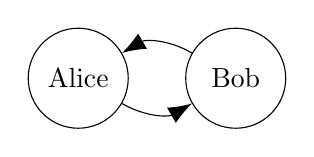
\begin{tikzpicture}[node distance=2cm,on grid, auto]
    \node[state,minimum size=0.5in] (alice) {Alice};
    \node[state,minimum size=0.5in] (bob) [right of=alice] {Bob};

    \path[-{Latex[length=3mm]}] (alice) edge [bend right] (bob)
              (bob)   edge [bend right] (alice);
  \end{tikzpicture}\\
  \textit{The only possible network with two members.}
\end{center}

In the case of three people, it gets more interesting. If we know two of the relationships, then the third must be known, since there is only one person not yet receiving a gift, and one person not yet supplying one. If we know only one, however, we run into a fork. Let our three people be Alice, Bob, and Carol. Without loss of generality\footnote{This is a really handy phrase for these sorts of hypotheticals. Essentially, what I mean by this is that the names are not important, and that we could instead choose to the names differently to represent any choice of initially known relationship. We might say instead that all cases are isomorphic to each other, but that takes longer.}, let us say that we know that Alice is giving Bob a gift. If Bob is giving Alice a gift, then Carol has no targets other than herself for gift-giving. This is disallowed, so knowing that Alice is giving Bob a gift must imply that Bob's gift is going to Carol. Only Alice remains as a gift-giving target, so Carol's gift must be going to her.\\

\begin{center}
  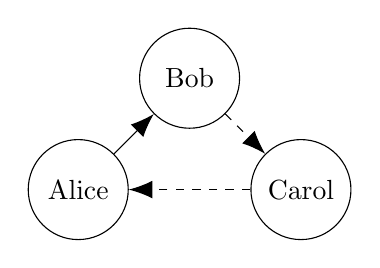
\begin{tikzpicture}[node distance=2cm,on grid,auto]
    \node[state,minimum size=0.5in] (alice) {Alice};
    \node[state,minimum size=0.5in] (bob) [above right of=alice] {Bob};
    \node[state,minimum size=0.5in] (carol) [below right of=bob] {Carol};

    \path[-{Latex[length=3mm]}] (alice) edge (bob);
    \path[-{Latex[length=3mm]},dashed] (bob) edge (carol)
                     (carol) edge (alice);
  \end{tikzpicture}\\
  \textit{Solid arrows are known, dashed arrows are inferred.}
\end{center}

In the case of four people (adding Dave to the mix), knowing one relationship is insufficient. We say without loss of generality again that we know that Alice is giving Bob a gift. Bob could then be giving a gift to Alice, leaving Carol and Dave to exchange gifts, or Bob could be giving a gift to Carol, leaving Dave to give Alice her gift. Other cases might be possible (for example, Bob could be giving to Dave) but having two is enough to demonstrate that we cannot solve a four person network by knowing only one relationship.\\

\begin{center}
  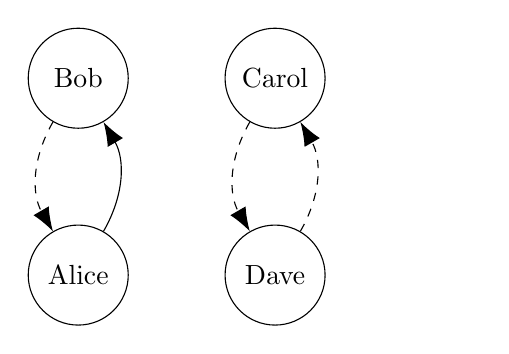
\begin{tikzpicture}[node distance=2.5cm,on grid,auto]
    \node[state,minimum size=0.5in] (alice) {Alice};
    \node[state,minimum size=0.5in] (bob) [above of=alice] {Bob};
    \node[state,minimum size=0.5in] (carol) [right of=bob] {Carol};
    \node[state,minimum size=0.5in] (dave) [below of=carol] {Dave};
    \node (empty) [right of=dave] {};

    \path[-{Latex[length=3mm]}] (alice) edge [bend right] (bob);
    \path[-{Latex[length=3mm]},dashed] (bob) edge [bend right] (alice)
                                       (carol) edge [bend right] (dave)
                                       (dave) edge [bend right] (carol);
  \end{tikzpicture}\hspace{2in}
  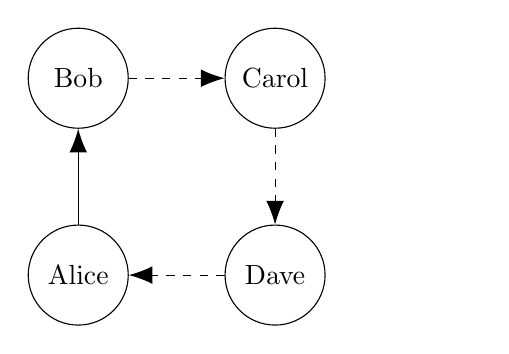
\begin{tikzpicture}[node distance=2.5cm,on grid,auto]
    \node[state,minimum size=0.5in] (alice) {Alice};
    \node[state,minimum size=0.5in] (bob) [above of=alice] {Bob};
    \node[state,minimum size=0.5in] (carol) [right of=bob] {Carol};
    \node[state,minimum size=0.5in] (dave) [below of=carol] {Dave};
    \node (empty) [right of=dave] {};
    
    \path[-{Latex[length=3mm]}] (alice) edge (bob);
    \path[-{Latex[length=3mm]},dashed] (bob) edge (carol)
                                       (carol) edge (dave)
                                       (dave) edge (alice);
    
  \end{tikzpicture}\hspace{2in}
  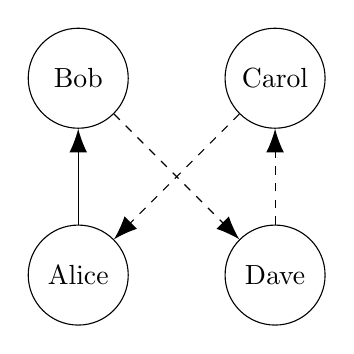
\begin{tikzpicture}[node distance=2.5cm,on grid,auto]
    \node[state,minimum size=0.5in] (alice) {Alice};
    \node[state,minimum size=0.5in] (bob) [above of=alice] {Bob};
    \node[state,minimum size=0.5in] (carol) [right of=bob] {Carol};
    \node[state,minimum size=0.5in] (dave) [below of=carol] {Dave};
    
    \path[-{Latex[length=3mm]}] (alice) edge (bob);
    \path[-{Latex[length=3mm]},dashed] (bob) edge (dave)
                                       (dave) edge (carol)
                                       (carol) edge (alice);
  \end{tikzpicture}\\
  \textit{Three posibilities when Alice $\rightarrow$ Bob}
  %[Secret santa network with n = 4, three possible cases.]
\end{center}

If we know two relationships, then can we solve the network? If Bob is giving Alice a gift in return, then yes, since the rest of the network is just another instance of the two person case. However, if Bob chooses to give a gift to (without loss of generality) Carol, then there remain two possible targets for Carol: Alice and Dave. If she gives to Alice, however, then Dave is both the last person without a gift, and without a gift-giving target. So she has to be giving to Dave. So knowing two relationships was sufficient to infer the remaining two.\\

\textit{Edited to add:} my brother pointed out, after reading this, a case where knowing two edges does not help you: when you know two edges that are disconnected, you do not know whether this is because there are two isolated pairs of gift exchangers, or one cycle containing all of the members. So the number of relationships you need to know for the four person case is three.\\

At this point, a pattern has emerged. We can see that in all cases, the valid networks have cycles\footnote{By cycle, we here mean a chain of gift-giving relationships where you eventually return to the start of the chain.} in them. Not everyone is necessarily included in every cycle: for example look at the case in the four person network where Alice and Bob are exchanging gifts independently of Carol and Dave's exchange. Is this a property that all networks must uphold? In order to answer a question like that, we can try to construct a counterexample. Either we succeed, and we demonstrate that the claim is false, or we fail, and hopefully do so in such a way as to motivate a proof that failure was inevitable.\\

What would a network where someone was not part of a cycle look like? We would have to be able to traverse gift-giving relationships to get from one person to another, but not back. Let us say that Alice is giving a gift to Bob (or possibly to someone who is giving a gift to Bob, and so on.) Bob cannot give a gift to any member of the chain of gift-givers leading between Alice and himself, because each of those people is receiving a gift from the previous person in the chain. He cannot give a gift to Alice, since then he would be completing a cycle. So he must give a gift to someone who has not yet been described, unless there are no people left. If there are no people left, then we are done. We have to form a cycle by giving to Alice. Otherwise, we can pick a new person for Bob to give a gift to from the remaining pool. This person, however, cannot give to Bob, or any of the other people in the chain, and he cannot give to Alice. We can call him the new Bob, and now we have the same situation as before, except there is one less person in the pool of people who have not yet been gift recipients. By induction, we know that eventually one of the remaining people must return to Alice\footnote{Incidentally, this result is something that I remember proving in a graph theory class, towards the beginning of a semester. This is why knowing some math is helpful in deriving more math. Oftentimes you can skip steps in your proof by describing them in terms of an existing theorem and then leveraging that result without having to re-proving it.}. We can repeat this process of extending the chain until the pool of free people is empty.\\

This tells us that if Alice can reach Bob by a chain of gift-giving, then Bob can reach Alice as well, for any ``Alice'' and ``Bob'' in the network. So all secret santa networks must contain one or more cycles. How, if at all, is this useful? The nice thing about cycles is that we can add an additional person to a cycle by taking one relationship, for example Carol $\rightarrow$ Dave, and simply inserting our interloper, Ellen, in the middle of it, getting Carol $\rightarrow$ Ellen $\rightarrow$ Dave. So if we cannot solve a particular network, we can always make it bigger without increasing the number of unknown---but derivable---edges by adding more known relationships to the network in a known part of the cycle. We can also introduce an independent cycle to the graph, all of which we know, and none of which helps us with the unknown parts.\\

In the four person case, we ran into trouble because Carol and Dave were interchangeable. We can construct an equivalent case with five people by adding Ellen in between Alice and Bob. For six people (adding Finn) we can split off Ellen and Finn into their own cycle, and get stuck with the same four person Alice, Bob, Carol and Dave network. We can then add as many people as we want to the Ellen and Finn network without affecting our inability to solve the four person cycle.\\

\begin{center}
  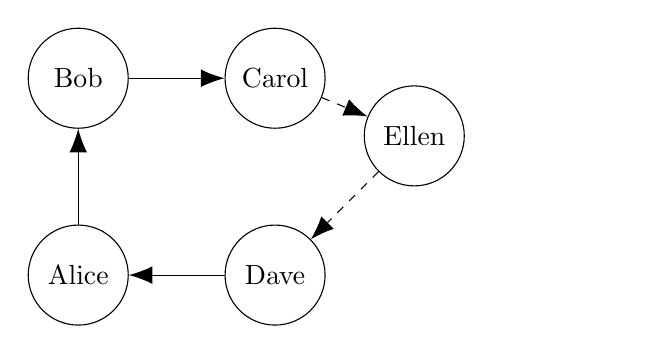
\begin{tikzpicture}[node distance=2.5cm,on grid,auto]
    \node[state,minimum size=0.5in] (alice) {Alice};
    \node[state,minimum size=0.5in] (bob) [above of=alice] {Bob};
    \node[state,minimum size=0.5in] (carol) [right of=bob] {Carol};
    \node[state,minimum size=0.5in] (dave) [below of=carol] {Dave};
    \node[state,minimum size=0.5in] (ellen) [above right of=dave] {Ellen};
    \node (empty) [right of=ellen] {};

    
    \path[-{Latex[length=3mm]}] (alice) edge (bob)
                                (bob) edge (carol)
                                (dave) edge (alice);
    \path[-{Latex[length=3mm]},dashed] (carol) edge (ellen)
                                       (ellen) edge (dave);
    
  \end{tikzpicture}\hspace{2in}
  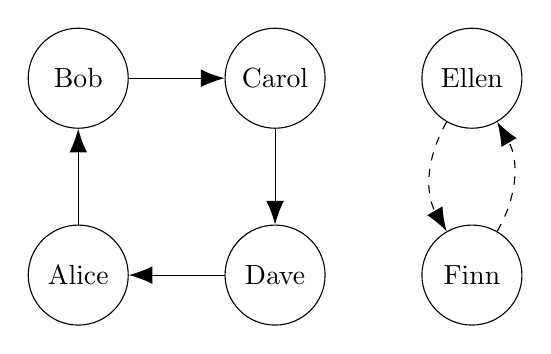
\begin{tikzpicture}[node distance=2.5cm,on grid,auto]
    \node[state,minimum size=0.5in] (alice) {Alice};
    \node[state,minimum size=0.5in] (bob) [above of=alice] {Bob};
    \node[state,minimum size=0.5in] (carol) [right of=bob] {Carol};
    \node[state,minimum size=0.5in] (dave) [below of=carol] {Dave};
    \node[state,minimum size=0.5in] (ellen) [right of=carol] {Ellen};
    \node[state,minimum size=0.5in] (finn) [right of=dave] {Finn};
    
    \path[-{Latex[length=3mm]}] (alice) edge (bob)
                                (bob) edge (carol)
                                (carol) edge (dave)
                                (dave) edge (alice);
    \path[-{Latex[length=3mm]},dashed] (ellen) edge [bend right] (finn)
                                       (finn) edge [bend right] (ellen);
  \end{tikzpicture}\\
  \textit{Adding Ellen and Finn to our four person network.}
\end{center}

So, for any network greater than four people, the number of relationships that can be unknown in a solvable network is the same as the number of relationships that can be unknown in a four person network. Which, as we discovered above, is two.\\

To recap, we tried to formalize the problem, tried some small cases until we hit an interesting pattern, proved that the pattern held using induction, and then used that pattern to answer the question, again using induction. If we had gotten stuck on the proof of the pattern, we could have gone into the literature and found a proof, since we had a mathematical model for the problem. I will leave you with an exercise: how does disallowing relationships with return gifts, for example where Alice gives Bob a gift, and then Bob gives Alice a return gift, affect our answer?\\
\end{document}
